In this last part, the test cases correspond to a two-phase flow at the most local scale.\newline
Two single-phase phases are separated by a mobile interface. The direct numerical simulation of these flows consists in numerically simulating all the spatio-temporal scales of the flow.
All inclusions (bubbles or drops) in the flow are described individually and the main difficulty is to follow finely these mobile interfaces with in particular fine adjustment of the remeshing 
parameters during the calculation. \medskip \newline
Several numerical methods allow such monitoring. The method used for the modeling of the \textbf{oscillating bubble} and \textbf{hanging drop} problems which will be treated in this part is the Front-Tracking method.
By this method, the front (interface) between fluids is followed by the computational grid.\medskip \bigskip  \newline
\begin{center}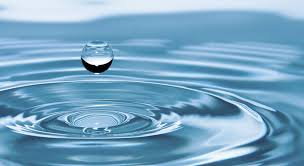
\includegraphics[width=12cm]{tools/goutte.png}\end{center}
